\documentclass[a4paper]{article}

\usepackage{url}
\usepackage{graphicx}
\usepackage{a4wide}

\title{\textbf{Pneumonia Detection using a CNN}}
\author{Bram Pulles -- S1015194}

\begin{document}
\maketitle

\section{Introduction}

Pneumonia is a serious lung condition responsible for the deaths of millions
each year. Diagnoses are often performed through the analysis of chest X-ray
images, due to its wide spread availability and relative low cost. AI can be
used to help professionals get to a diagnosis. In this report we outline a
computer vision method using convolutional neural networks (CNN) to detect
pneumonia.

Much research has gone into computer aided pneumonia detection. We take the
existing research done by Szepesi, et al (2022) and reimplement their
architecture. In contrast to other approaches using transfer learning, they
focus on a simple CNN that was not pre-trained. Their research is unique,
because they add a dropout layer to a convolutional block, which is
unconventional. We will use their results to set the optimal parameters of our
network.

In section \ref{sec: methods} we dive into the inner workings of our CNN, as
well as the dataset, learning procedure and evaluation criteria of our model.
We will discuss the architecture in detail and outline the parameter settings
that we use. In section \ref{sec: results} we discuss the performance of the
CNN on the training data and relate these to various measures. In section
\ref{sec: discussion} we conclude with a critical review to our study and
findings.

\section{Methods}\label{sec: methods}

\subsection{Dataset}

The dataset on which we train the CNN is provided through a Kaggle
competition\footnote{\url{https://www.kaggle.com/datasets/paultimothymooney/chest-xray-pneumonia}}.
It contains a total of 5863 chest X-ray images, labeled as either normal or
pneumonia. The images are taken of pediatric patients of one to five years old
from Guangzhou Women and Children's Medical Center. All images are taken as
part of routine patient clinical care. The images have been filtered before
being admitted to the dataset by removing low quality images. The labels for
the images are determined by two expert physicians. In addition, a third expert
has checked the labels for errors.

Szepesi, et al (2022) uses the same dataset. However, they use additional
images for training made by generative AI. The images are generated for the
pneumonia labeled cases as these are less common in the data. We do not
generate extra images in this way. Instead we use a simple data generator which
performs tranformations on the images to generate extra data. In particular, we
randomly rotate the images by at most 30 degrees, zoom in by at most 20\%,
shift in height and width by at most 10\% and randomly flip the images
left-right. Of course, we also normalize the data to value between 0 and 1 by
dividing through 255. At last, we resize the images to a size of 224 by 224 to
be in line with Szepesi, et al (2022) and other literature.

Originally, the dataset is split into a train, test and validation set, where
the latter only contains a total of 16 samples. We resample the data such that
it is a 80\%/10\%/10\% split. This way we can actually use the validation set
and test the generalisation behaviour of our model with statistical
significance. As this problem applied to more people on Kaggle we use the
snippet provided by Mahdi Ravaghi to perform this reshuffling of the
data\footnote{\url{https://www.kaggle.com/datasets/paultimothymooney/chest-xray-pneumonia/discussion/485689}}.
The distribution of samples after the resampling can be seen in figure
\ref{fig: dataset}.

\begin{figure}[h]
	\centering
	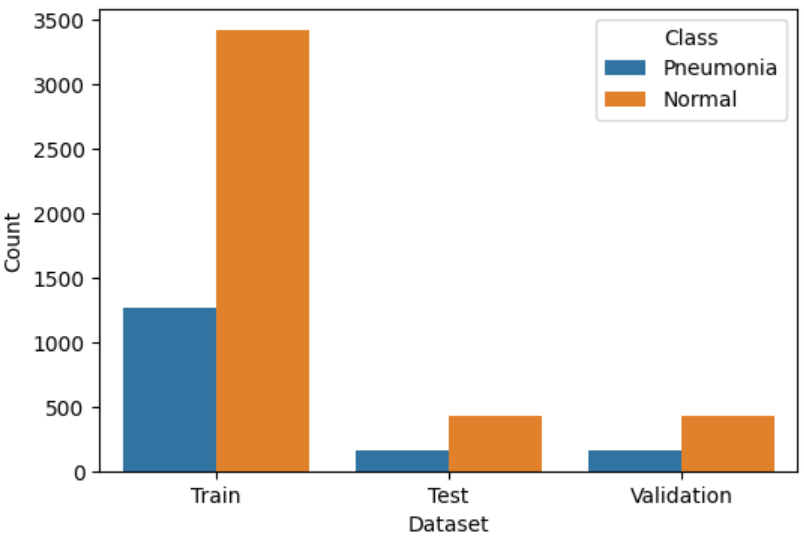
\includegraphics[width = 0.5\textwidth]{imgs/dataset.png}
	\caption{The dataset sample count after the 80\%/10\%/10\% split.}
	\label{fig: dataset}
\end{figure}

\subsection{Model}

An impression of a similar model architecture can be seen in figure \ref{fig:
model}. As visible, it consists of several chained convolutional blocks. In our
model there are five blocks each consisting of two convolutions both followed
by a batch normalisation and ReLU activation layer. The batch normalisation
layers normalize the inputs for the next layer helping to stabilize learning,
reaching convergence more quickly and introducing a bit of noise which can have
a slightly regularizing effect. The convolution kernels are of size 3 by 3, use
zero padding to maintain spatial dimensions and do not use biases. Each
convolutional block is ended with a max pooling of 2 by 2 or 3 by 3 to
summarize the feature maps provided by the convolutional layers.

\begin{figure}[h]
	\centering
	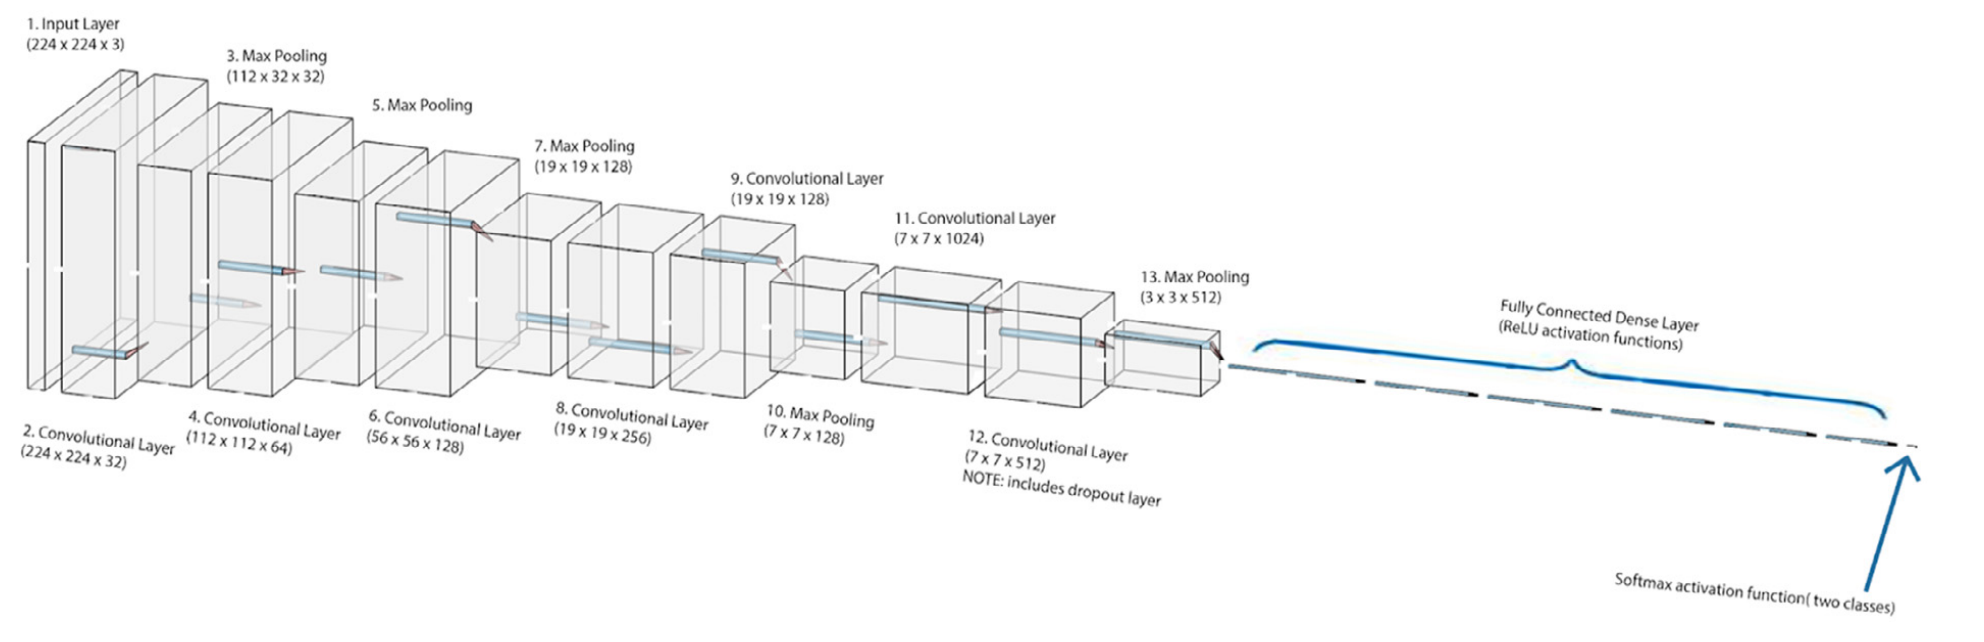
\includegraphics[width = \textwidth]{imgs/model.png}
	\caption{Structure of the model from Szepesi, et al (2022).}
	\label{fig: model}
\end{figure}

Before the chained convolutional blocks there is the input layer. This input
layer takes the three channeled RGB encoded images and passes it straight to
the first block. After the five blocks there is a flattening layer followed by
a series of densely connected layers with ReLU activation functions in between.
This fully connected dense set of layers operates on the feature maps provided
by the convolutional blocks before and determines whether there is pneumonia or
not. In the final output layer we have two output nodes on which we perform the
softmax operation to get a probability for each label. In appendix \ref{app:
model} a full specification of all layers is given.

Importantly, Szepesi, et al (2022) introduces the unique integration of a
dropout layer in the fifth convolutional block. The dropout occurs after the
second convolutional layer, but before the batch normalisation step. They found
that a dropout rate of 0.4 performs best, which is what we use as well. The
dropout layer regularizes the network and prevents it from becoming over dependent on
a small number of variables.

\subsection{Learning}

The loss which we optimize for is defined as the categorical cross entropy on
the validation set, an obvious choice for our problem. We use the Adam
optimizer with a learning rate of 1e-4. However, this learning rate is not
static. As the model improves it can be beneficial to lower the learning rate
to make smaller more accurate steps and avoid overshooting. To this end, we use
a learning rate reduction, on par with Szepesi, et al (2022). If the validation
loss does not improve for 5~epochs, we lower the learning rate by a factor
of 0.8 to a maximum of 1e-6. If the validation loss does not improve over 15
epochs we stop and call it done. When we do not stop early, we perform a
total of 50 epochs.

\subsection{Evaluation}

After training we evaluate the model performance using a few metrics. We
evaluate the accuracy and loss over time (for each epoch) on both the train and
validation datasets. Using the test set, we also compute a confusion matrix,
describing the rate of true positive, true negative, false positive and false
negative predictions. Especially, false positive and false negative evaluations
are important in the medical realm, as you do not want to do a medical
procedure on a healthy patient, or, not do a procedure on a sick patient.
Precision and recall on the test set allow us to get an even better image of
these properties.

\section{Results}\label{sec: results}

The training and validation accuracy and loss over time are visualised in
figure \ref{fig: history}. From these figures we can see that the training
accuracy and loss follow a very stable trajectory. This is good, it suggests we
chose good values for the learning rate over time. We also see that the
validation accuracy and loss is less stable, but seems to get more stable over
time. The validation set measures the generalisable performance of the model
and it makes sense that this is not as stable at the start. It is promising
that it stabilises over time, this is desired behaviour. Overall, it would be
good to run the training for more epochs, however, this already takes about 3
hours.

\begin{figure}[h]
	\centering
	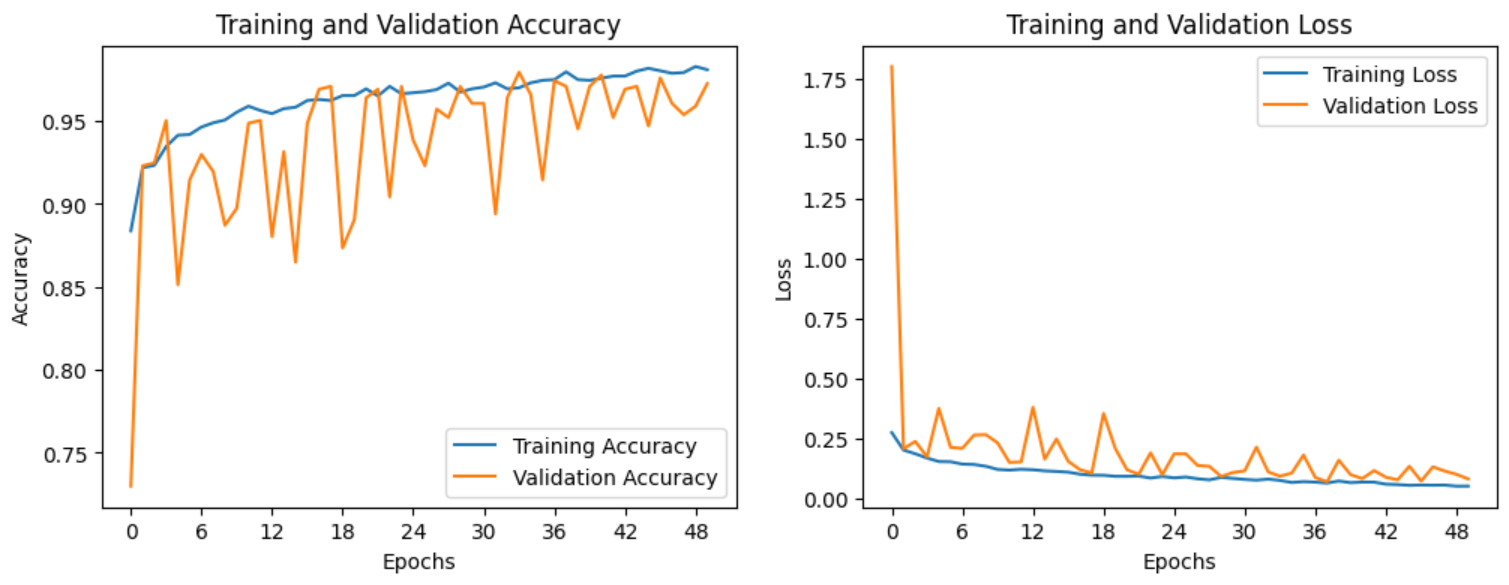
\includegraphics[width = \textwidth]{imgs/history.png}
	\caption{Accuracy and loss over time for the training and validation sets.}
	\label{fig: history}
\end{figure}

The confusion matrix is visualised in figure \ref{fig: confusion matrix}. From
this confusion matrix we can derive all our metrics as seen in table \ref{tab:
metrics}. Additionally, we achieved an accuracy of 95.91\% on the test set.
Overall, these results are very good and close to the results in Szepesi, et al
(2022). The precision on the pneumonia class is a bit lower, this can probably
be explained by the imbalance in the number of test cases available for each
class. The original paper solved this issue with using generative AI to create
an even amount of images, we did not use this approach.

\begin{figure}[h]
	\centering
	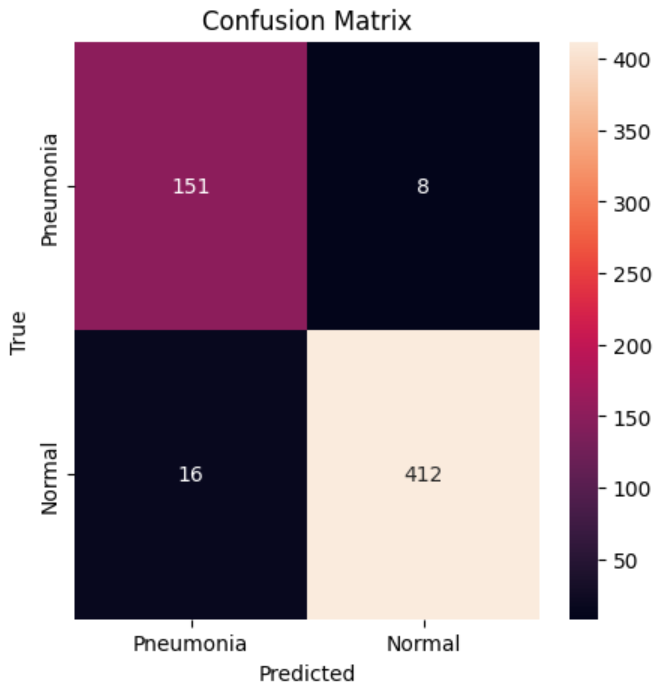
\includegraphics[width = .5\textwidth]{imgs/confusion_matrix.png}
	\caption{Confusion Matrix for the final model on the test set.}
	\label{fig: confusion matrix}
\end{figure}

\begin{table}[h]
	\centering
	\begin{tabular}{|c|c|c|c|c|}\hline
	            & precision& recall& support \\\hline
	   Pneumonia&      0.90&   0.95&     159 \\\hline
	      Normal&      0.98&   0.96&     428 \\\hline
	\end{tabular}
	\caption{Metrics of the final model on the test set.}
	\label{tab: metrics}
\end{table}

\section{Discussion}\label{sec: discussion}

We have seen in this report how a CNN model as proposed by Szepesi, et al
(2022) can be implemented and how it performs under slightly different
circumstances. The CNN model accurately distinguishes X-ray images of pneumonia
and normal lungs. The model achieves high precision and recall, most metrics
being close to other state of the art solutions.

For the future, we can likely improve the performance further by increasing the
number of epochs. We can also work on the data imbalance by generating or
retrieving more pneumonia lung images. It would also be interesting to do a
hyperparameter search on the model architecture, but this would be very
computationally heavy. Overall, the performance of the current model is already
excellent, but there are ideas to make it even better.

\section*{References}

\begin{itemize}
	\item
		Patrik Szepesi, László Szilágyi, Detection of pneumonia using
		convolutional neural networks and deep learning, Biocybernetics and
		Biomedical Engineering, Volume 42, Issue 3, 2022, Pages 1012-1022, ISSN
		0208-5216, \url{https://doi.org/10.1016/j.bbe.2022.08.001}.
\end{itemize}

\appendix

\pagebreak
\section{Model}\label{app: model}

\begin{figure}[h]
	\centering
	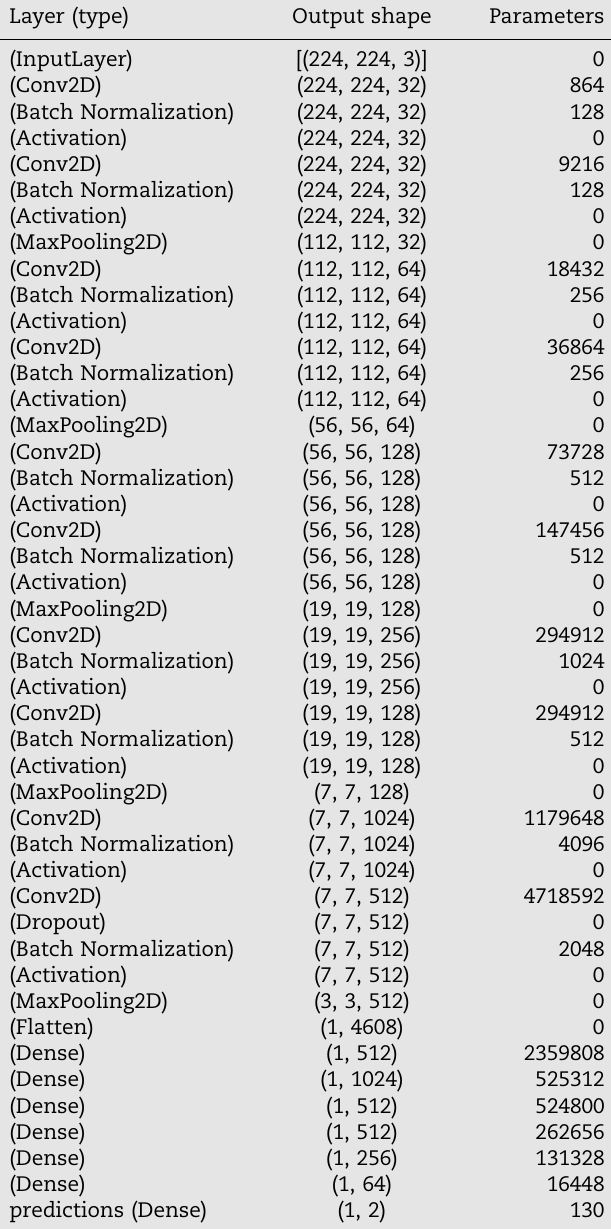
\includegraphics[width = 0.5\textwidth]{imgs/specs.png}
	\caption{Model specification details, same as in Szepesi, et al (2022).}
	\label{fig: specs}
\end{figure}


\end{document}
